\chapter{Performance Evaluation and Analysis}

\section{Experiment Setup}

In Figure~\ref{fig:diff_images} we ran different solvers on the same input image to compare them visually, as well as in terms of time and memory efficiency. All solvers used the same image preprocessing and the same drawing algorithm (Xiaolin-Wu). Solvers (a) through (h) used 128 pegs, while solver (i) used 256. Increasing the number of pegs for all solvers either results in incorrect line selection (due to naive line selection methods) or significantly higher computation time.

Solver (a) uses least squares with real coefficients. Solver (b) is a binary rounding of (a), using the top 1000 lines selected based on the coefficients from (a). Solver (c) constrains coefficients to lie within \(\left[0, 1\right]\) and selects 1000 lines. Solver (d) is a binarization of (c), using supersampling with \(\sigma=4\).

Solver (e) is a regularized version of least squares. Solver (f) is binary projection least squares. Solvers (g) and (h) both use orthogonal matching pursuit with 1000 line selections: (g) with real coefficients and (h) in binary form, the latter employing supersampling with \(\sigma=4\).

Finally, solver (i) is the Radon solver, which allows unlimited lines but includes an early stopping mechanism and uses \(\sigma=8\)

\section{Benchmarks}

\begin{table}[!ht]
\centering
\caption{Computation Time, Peak Memory Usage, and RMS of Different Solvers}
\begin{tabularx}{\textwidth}{l C C C}
\toprule
\textbf{Solver} & \textbf{Computation Time (s)} & \textbf{Peak Memory Usage (MB)} & \textbf{RMS} \\
\midrule
(a) ls     &    32.531          &   \textbf{321.970} & 0.1530          \\
(b) ls     &    \textbf{31.640} &   \textbf{321.970} & 0.2933          \\
(c) lls    &   169.719          &   770.275          & 0.3243          \\
(d) lls    &   172.250          &   770.273          & 0.2255          \\
(e) lsr    &   324.468          &  9596.899          & \textbf{0.1488} \\
(f) bpls   & 14499.700          & 10112.366          & 0.4447          \\
(g) mp     &    59.464          &  2762.394          & 0.2427          \\
(h) mp     &   158.776          &  1242.166          & 0.2339          \\
(i) radon  &  2170.854          &  1255.895          & 0.1807          \\
\bottomrule
\end{tabularx}
\end{table}

\begin{figure}[H]
    \centering
    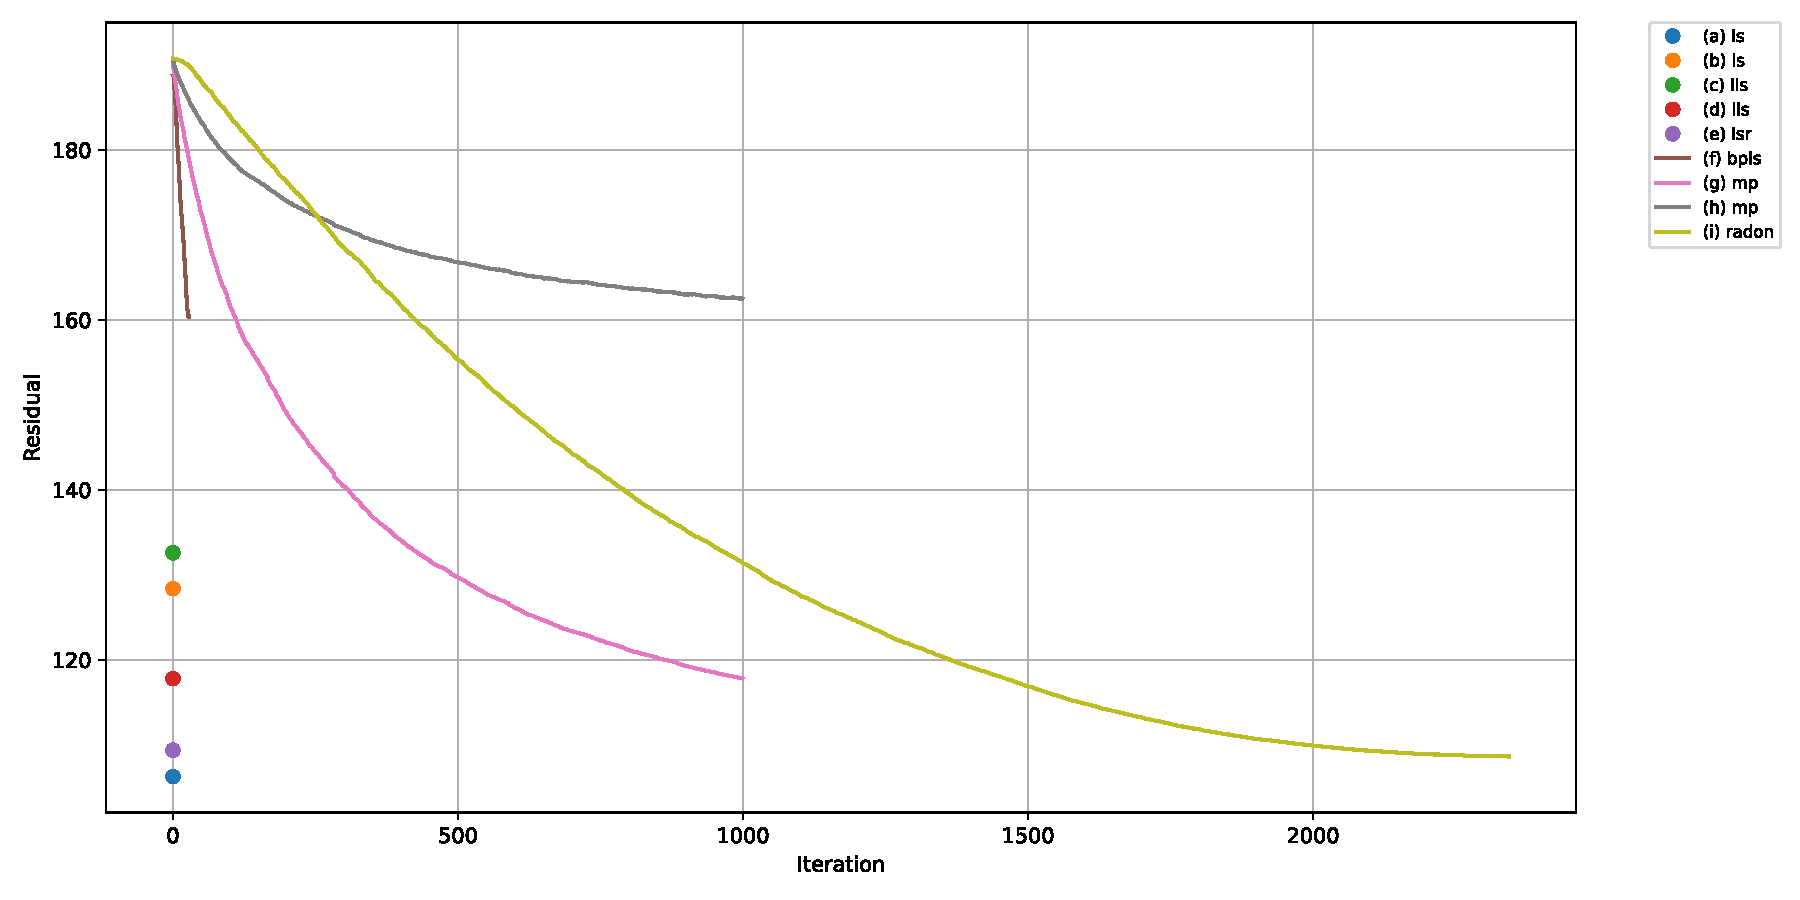
\includegraphics[width=\linewidth]{images/benchmarks/residual_history.pdf}
    \caption{Residual error over iterations for each solver.}
    \label{fig:residual_history}
\end{figure}

\section{Evaluation Summary}

The lowest RMS value belongs to (e) lsr, however, it is very close to (a) ls while being 10× slower and consuming 30× more memory. The RMS delta is negligible (\(\approx\)0.0042). Being the simplest, the (a) ls solver is both the fastest and the most memory efficient. However, its visual output is not desirable, we would prefer our best choice to be a binary solver. This narrows the candidates to (d), (f), (h), or (i). Among these, the best subjective image quality belongs to (d) LLS, while the best RMS score is achieved by (i) radon. One advantage of (i) radon is its ability to separate the subject from the background: the white areas are more prominent, and the overall line selection pattern appears more organized.

Looking at Figure~\ref{fig:residual_history}, we observe that (i) shows a slow, steady decrease in residuals. Other solvers, like (f), drop more aggressively, but this doesn’t necessarily yield better visual results. Among the iterative methods, (i) is the most stable and achieves the lowest residual error. Given these observations, along with its reasonable time and memory usage, we conclude it offers the best overall balance. To confirm this further, we compare it on another image:

\begin{figure}[H]
    \centering
    \begin{minipage}{0.2\linewidth}
        \centering
        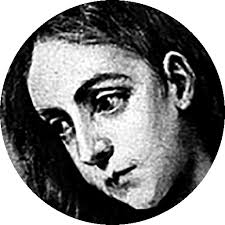
\includegraphics[width=\linewidth]{images/lls vs radon/mary.png}
    \end{minipage}
    \begin{minipage}{0.2\linewidth}
        \centering
        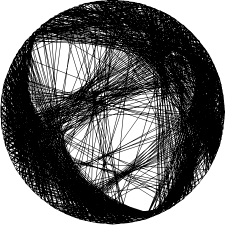
\includegraphics[width=\linewidth]{images/lls vs radon/lls.png}
    \end{minipage}
    \begin{minipage}{0.2\linewidth}
        \centering
        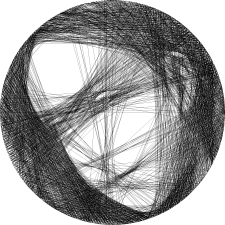
\includegraphics[width=\linewidth]{images/lls vs radon/radon.png}
    \end{minipage}
    \caption{Comparative analysis between (d) lls (center) and (i) radon (right), with input image (left).}
    \label{fig:lls_vs_radon}
\end{figure}

\begin{figure}[H]
    \centering
    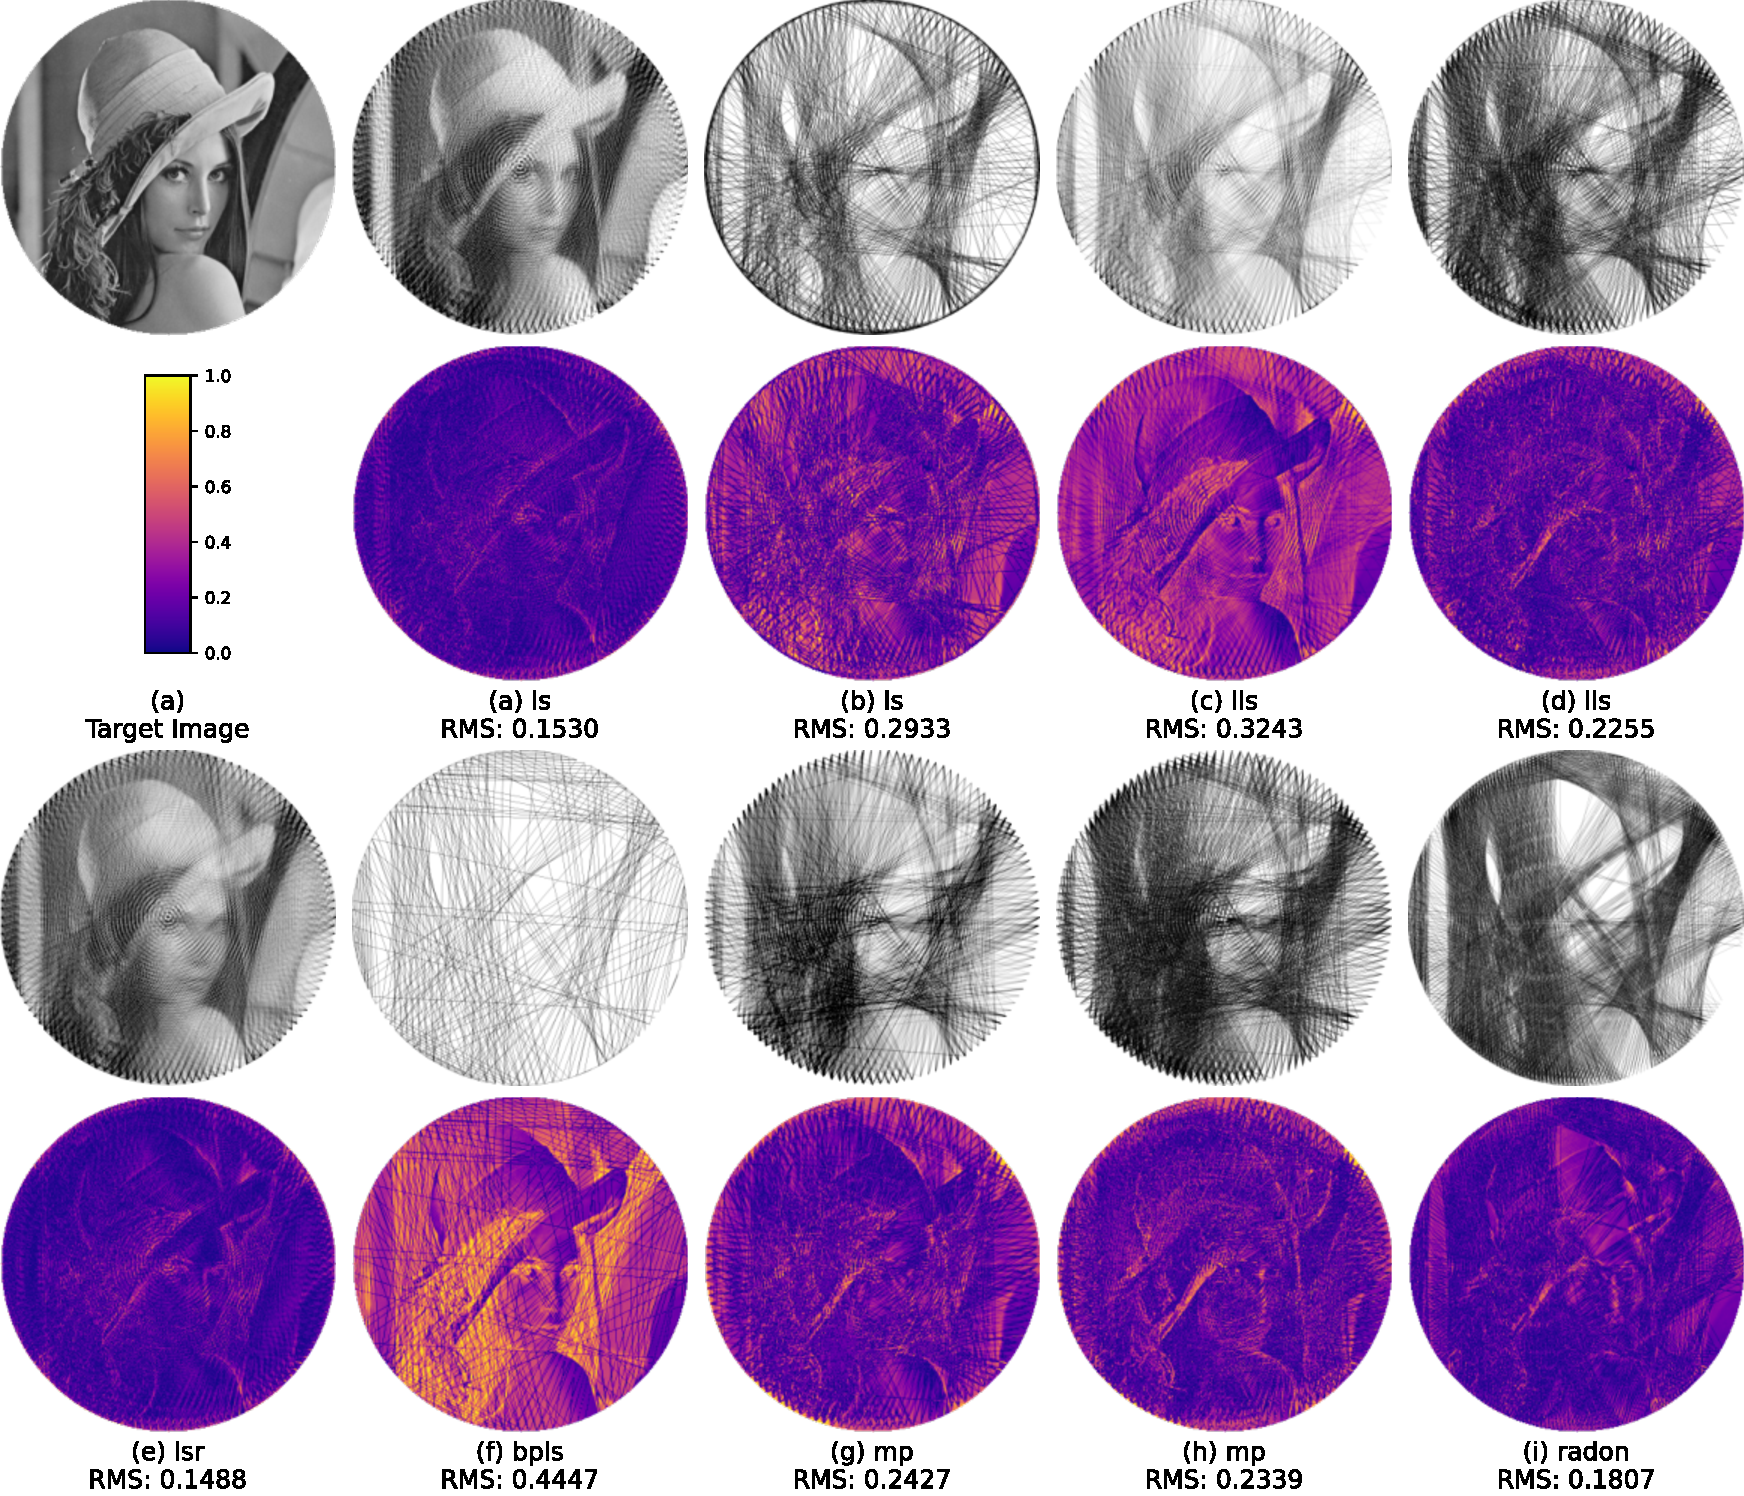
\includegraphics[width=0.9\linewidth]{images/benchmarks/diff_images.pdf}
    \caption{Comparative analysis of the results produced by different solvers. The first image is the input target image, and for each solver, we display the reconstructed image alongside the absolute difference image with respect to the target.}
    \label{fig:diff_images}
\end{figure}
